\documentclass[a4paper]{article}

%% Language and font encodings
\usepackage[english]{babel}
\usepackage[utf8x]{inputenc}
\usepackage[T1]{fontenc}

%% Sets page size and margins
\usepackage[a4paper,top=3cm,bottom=2cm,left=3cm,right=3cm,marginparwidth=1.75cm]{geometry}

%% Useful packages
\usepackage{amsmath}
\usepackage{graphicx}
\usepackage[colorinlistoftodos]{todonotes}
\usepackage[colorlinks=true, allcolors=blue]{hyperref}
\usepackage{float}
\usepackage{verbatim}

\title{Ph 20 Lab3 Write Up}
\author{Yuankun David Wang}

\begin{document}
\maketitle


\section{Part 1}
\subsection{The Explicit Euler Method}
The following plots show the numerically integrated solution to a simple harmonic oscillator with initial conditions x = 1 and v = 0. 
For the explicit Euler method, the errors vary periodically, with increasing amplitude. The amplitude of errors appears to increase exponentially (not picture, but for many cycles this becomes more apparent). The long range trend for the total energy, which is proportional to $x^2 + v^2$ is a linear increase with time. Since we know that energy is conserved in the analytic solution, this increase in energy must be a result of the accumulation of errors due to small errors in the numerical integration.

\begin{figure}[H]
\centering
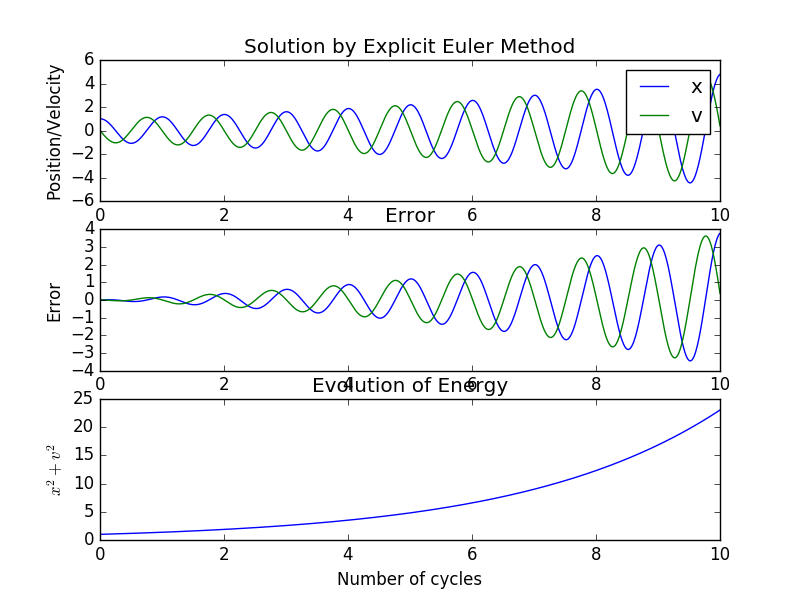
\includegraphics[width=0.7\textwidth]{expl.png}
\caption{\label{fig:expl}The first subplot shows the solutions for x and v obtained via numerical integration by the Explicit Euler method. The second subplot shows the errors that accumulate. The third plot shows the evolution of the energy in the system, which increases linearly with time due to the accumulation of errors. The value of h used while integrating was .01}
\end{figure}

\subsection{Truncation Error}
The truncation error is plotted as a function of h in figure 2. Note that the x-axis goes from larger h to smaller h, showing that the error decreases as h becomes smaller. The error becomes much better as h becomes smaller, as is roughly proportional to h.

\begin{figure}[H]
\centering
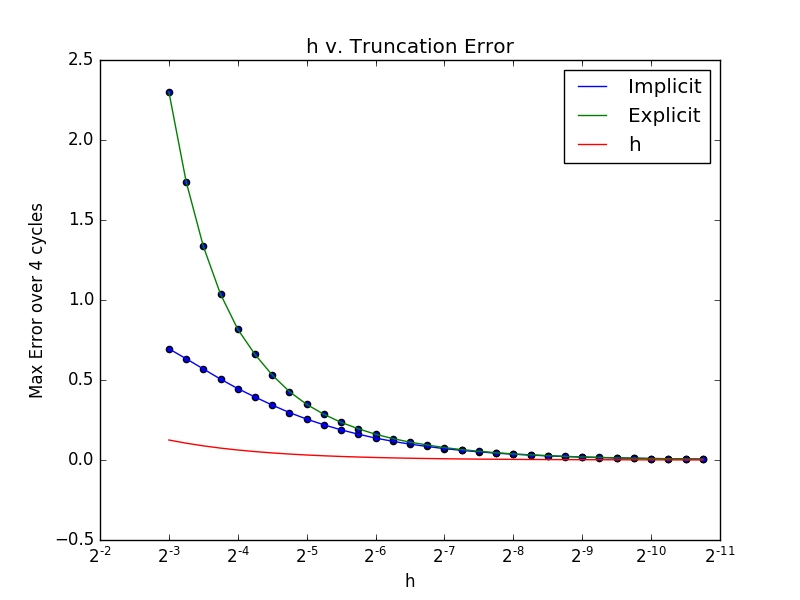
\includegraphics[width=0.7\textwidth]{t_err.png}
\caption{\label{fig:t_err}The truncation error associated with implicit and explicit Euler methods, as a function of h. Note that as h becomes small, the truncation error goes approximately as h.}
\end{figure}

\subsection{The Implicit Euler Method}
The solution to the propagation of the implicit Euler method was found by taking the inverse of the matrix found in Equ 7 in the notes. The errors appear to increase at the same rate, but flipped about the y-axis. This indicates that the small accumulations will decrease the amplitude of the estimate. This is confirmed by the Total energy plot, which decreases with the number of cycles.

\begin{figure}[H]
\centering
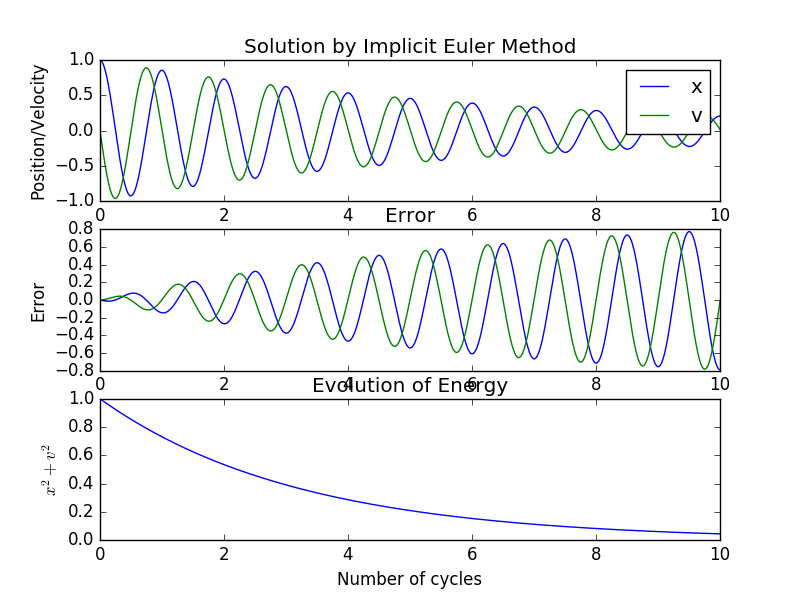
\includegraphics[width=0.7\textwidth]{impl.png}
\caption{\label{fig:expl}The first subplot shows the solutions for x and v obtained via numerical integration by the Implicit Euler method. The second subplot shows the errors that accumulate. The third plot shows the evolution of the energy in the system, which decreases linearly with time due to the accumulation of errors. The value of h used while integrating was .01}
\end{figure}

\section{Part 2}
\subsection{Phase Trajectories of the Explicit and Implicit Euler methods}
A perfect solution to the SHO would have a perfectly circular trajectory in phase space, given our in initial conditions (k, m = 1). We see that the numerically integrated solutions deviate from this. The energy of the system is proportional to the area enclosed by is trajectory in phase space. Note that this area decreases for the implicit method and increases for the explicit method as the trajectories spiral inwards or outwards.

\begin{figure}[H]
\centering
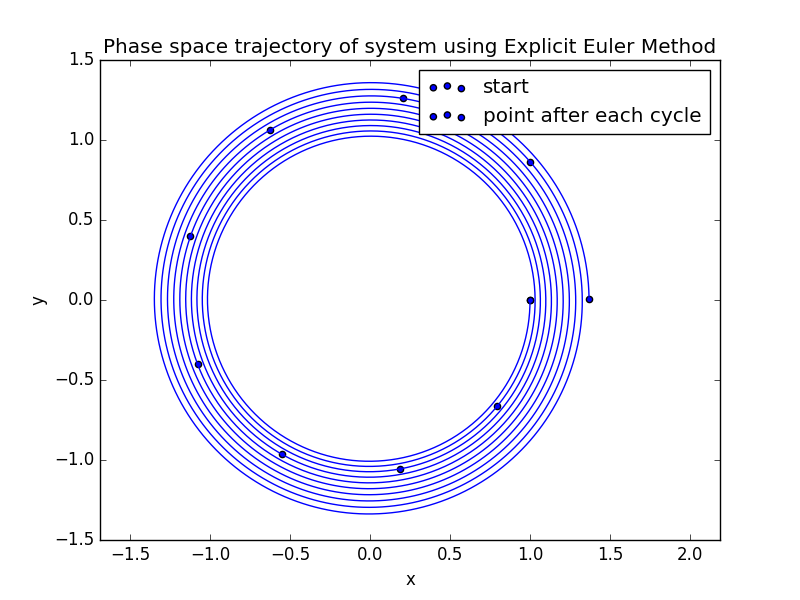
\includegraphics[width=0.7\textwidth]{ph_e.png}
\caption{\label{fig:ph_e}The plot of the first 4 cycles of the SHO in phase space, using the numerical solution obtained by the explicit Euler method. Note how the trajectory spirals outward. If energy were conserved, we would expect the trajectory to be closed. The starting point is noted with a blue dot. The interval h used was .01}
\end{figure}

\begin{figure}[H]
\centering
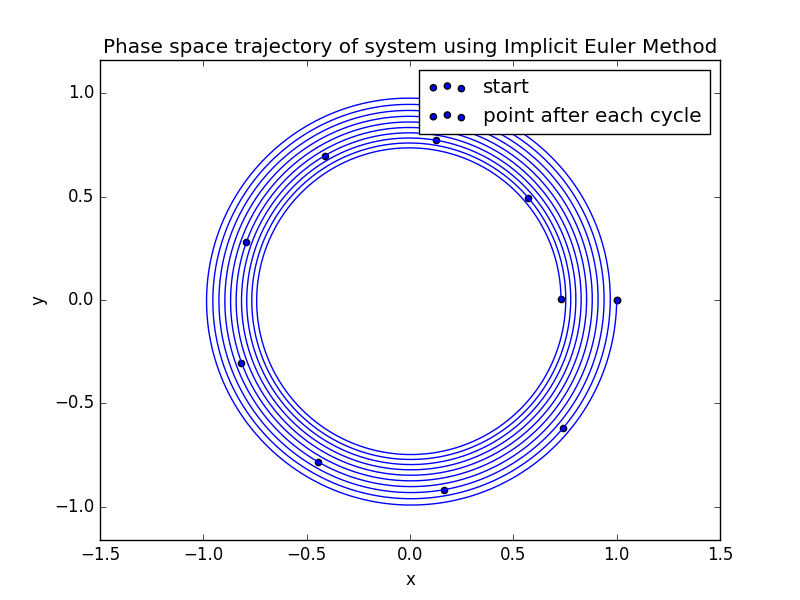
\includegraphics[width=0.7\textwidth]{ph_i.png}
\caption{\label{fig:ph_i}The plot of the first 4 cycles of the SHO in phase space, using the numerical solution obtained by the implicit Euler method. Note how the trajectory spirals inward. Again, the system is losing energy. The starting point is noted with a blue dot. The interval h used was .01}
\end{figure}

\subsection{The Symplectic Euler Method}
Here we see that the amplitudes are conserved, as the energy oscillates about 1 with a frequency roughly equal to the frequencies of x and v. However, upon closer examination, the frequency of oscillation lags slightly compared with that of the perfect solution. In figure[], the analytic and symplectic solutions with h=.1 after 100 cycles are plotted on the same axis. The sypmletic solution is almost 180 out of phase with the analytic solution!

\begin{figure}[H]
\centering
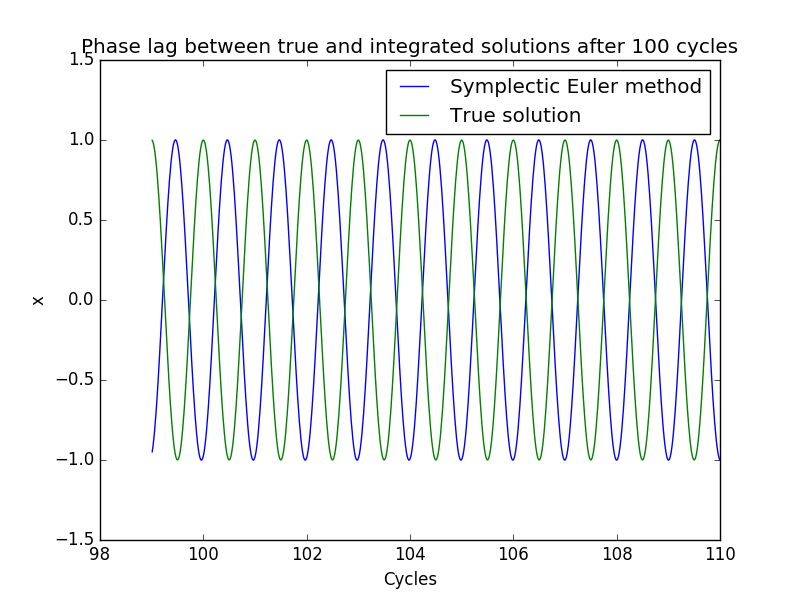
\includegraphics[width=0.7\textwidth]{lag.png}
\caption{\label{fig:lag}The lag between the numerical and analytical solutions after 100 cycles. The are almost completely out of phase. The integration was done using h = 0.1}
\end{figure}


\subsubsection{Phase Trajectory}
As expected, the plot of the phase trajectory of the symplectic solution is closed.


\begin{figure}[H]
\centering
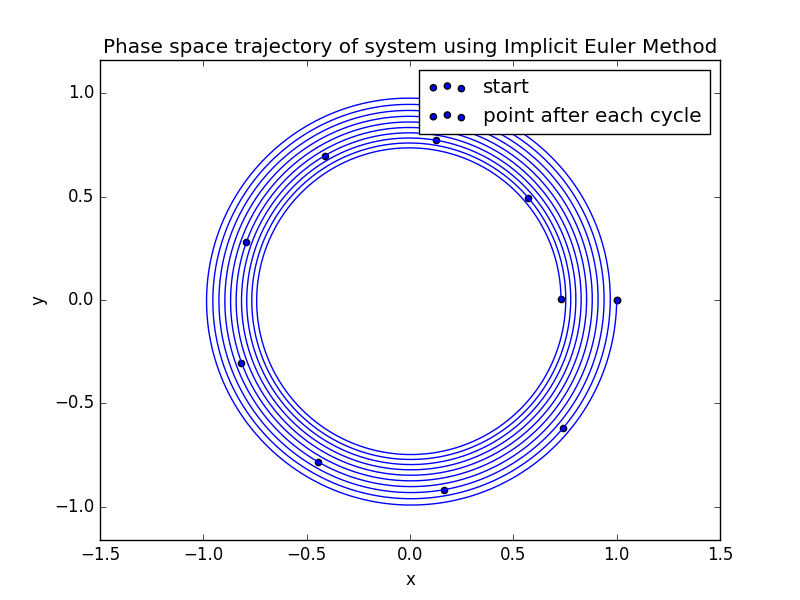
\includegraphics[width=0.7\textwidth]{ph_i.png}
\caption{\label{fig:ph_s}The plot of the first 4 cycles of the SHO in phase space, using the numerical solution obtained by the symplectic Euler method. Note how the trajectory appears closed. The starting point is noted with a blue dot. The interval h used was .01}
\end{figure}

\section{Documents}
\subsection{code}
\verbatiminput{functions.py}
\verbatiminput{main.py}
\subsection{Makefile}
\verbatiminput{Makefile}
\subsection{Logs and Output}
\verbatiminput{main.log}




\end{document}
